%%%%%%%%%%%%%%%%%%%%%%%%%%%%%%%%%%%%%%%%%%%%%%%%%%%%%%%%%%%%%%%%%%%%%%%%%%%%%%%%%%%%%%%%%%%%%%%%%%%
%%%%%%%%%%%%%%%%%%%%%%%%%%%%%%%%%%%%%%%%%%%%%%%%%%%%%%%%%%%%%%%%%%%%%%%%%%%%%%%%%%%%%%%%%%%%%%%%%%%
%%%%%%%%%%%%%%%%%%%%%%%%%%%%%%%%%%%%%%%%%%%%%%%%%%%%%%%%%%%%%%%%%%%%%%%%%%%%%%%%%%%%%%%%%%%%%%%%%%%
%%%%%%%%%%%%%%%%%%%%%%%%%%%%%%%%%%%%%%%%%%%%%%%%%%%%%%%%%%%%%%%%%%%%%%%%%%%%%%%%%%%%%%%%%%%%%%%%%%%

\chapter{Conceptos}

Para poder identificar marcadores significativos para el diagnóstico del deterioro cognitivo, 
éste debe ser estudiado desde la neuropsicología; dentro de ésta última se destaca la técnica de 
electroencefalografía, que es usada para medir cierto tipo de actividad cerebral y que 
posiblemente esté asociada al deterioro cognitivo. 
Una vez expuestos los conceptos pertinentes, se presenta una colección de objetos matemáticos
(procesos estocásticos débilmente estacionarios) con los cuales se han modelado un tipo de
actividad cerebral, y que fue comparado con mediciones de la misma.

La exposición se divide en dos subsecciones marcadamente diferentes: matemáticas y 
fisiología/psicología.
En la primera se menciona al deterioro cognitivo en adultos mayores, con énfasis en su 
caracterización dentro del sistema nervioso.
La segunda subsección se centra en las herramientas estadísticas utilizadas para analizar datos 
experimentales, entendidas no como simples \textit{técnicas} sino como objetos abstractos definidos 
formalmente.

Estas dos partes difieren no sólo en temas sino también epistemológicamente: en la primera aparecen 
afirmaciones basadas en datos experimentales, acompañadas de las citas pertinentes, mientras que en 
la segunda las afirmaciones son formalmente verdaderas y demostrables en el sistema axiomático 
usual. Respecto a estas últimas, varias de las demostraciones se presentan como apéndice junto las 
definiciones pertinentes, mientras otras son citadas debido a diversos motivos.

\section{Psicología}

%La demencia es un síndrome debido a la disfunción cerebral, que produce desintegración
%de la conducta en los planos intelectual y emocional, alterando significativamente la
%función social y laboral del paciente.
La \textbf{demencia} es, según el Manual diagnóstico de y estadístico de trastornos mentales 
(DSM-IV), \textit{un síndrome que consiste en el desarrollo de déficit cognoscitivos 
suficientemente graves como para interferir significativamente en las actividades laborales y 
sociales, respecto al nivel de actividad previo. 
%Aparece precedida por una enfermedad médica o el efecto de exposición prolongada a sustancias 
%tóxicas, incluso ambos.
Los sujetos con demencia tienen una baja capacidad para aprender información nueva y suelen olvidar 
lo aprendido anteriormente, siendo éste el síntoma más prominente} \cite{DCM5}.

Cuando un sujeto presenta cambios marcados en su conducta, es relativamente fácil identificar la 
demencia; caso contrario es el diagnóstico temprano de la misma, el cual es importante para un 
tratamiento adecuado que revierta o desacelere el avance de este síndrome.
Se ha señalado que los criterios del manual DSM-IV son suficientes para este diagnóstico
\cite{Knopman01}.

Considerando a los \textbf{adultos mayores}, entendidos como individuos de 60 años o más, conviene 
destacar que el envejecimiento es determinado por una serie de procesos moleculares, celulares, 
fisiológicos y psicológicos que conducen directamente al deterioro de funciones cognitivas, 
específicamente atención y memoria \cite{Navarrete03,Park09}.
La funcionalidad durante esta etapa se relaciona con el estilo de vida, los factores de riesgo, el 
acceso a la educación y las acciones para el cuidado de la salud realizadas en edades más 
tempranas \cite{Ohayon04,Sanhueza14}.

Al momento de diagnosticar deterioro cognitivo en adultos mayores, deben tenerse en cuenta el 
envejecimiento normal y la posible \textbf{pseudodemencia depresiva}, ya que presentan 
características similares. Con respecto a ésta última, definida como \textit{un trastorno del 
afecto y que produce un aparente deterioro cognitivo} \cite{DCM5}, aunque no es efectivamente un 
tipo de demencia bien puede desencadenar en ello en ausencia de un tratamiento adecuado.

Como es usual, se considerará como etapa precursora de la demencia al \textbf{deterioro cognitivo 
leve}, definido como \textit{un síndrome caracterizado por una alteración adquirida y prolongada de 
una o varias funciones cognitivas, que no corresponde a un síndrome focal y no cumple criterios 
suficientes de gravedad para ser calificada como demencia} \cite{Robles02}.
En el transcurso de este escrito este padecimiento será manejado como \textbf{posible deterioro 
cognitivo (PDC)} ya que el autor no tiene la autoridad ni la autorización para efectuar un 
diagnóstico clínico, y porque los síntomas en esta etapa se consideran --afortunadamente-- 
reversibles.

%%%%%%%%%%%%%%%%%%%%%%%%%%%%%%%%%%%%%%%%%%%%%%%%%%%%%%%%%%%%%%%%%%%%%%%%%%%%%%%%%%%%%%%%%%%%%%%%%%%

\subsection{Psicometría}

En psicología los instrumentos de medición estándar son las \textbf{pruebas neuropsicológicas}, 
entendidas como muestras de alguna conducta de interés a las que se asignan puntajes para comparar 
cuantitativamente entre sujetos \cite{Ardila12}.

Las habilidades medibles a través de test neuropsicológicas se suelen agrupar en áreas o 
\textbf{dominios}: atención, lenguaje, cálculo, memoria y aprendizaje, percepción, motricidad, 
funciones somatosensoriales, habilidades espaciales, funciones ejecutivas. Esta clasificación puede
variar según algunos autores.
%No  existe  un  manual  de  síndromes  neuropsicológicos,  aunque  muchos  de  ellos  se incluyen 
%en el Manual Diagnóstico y Estadístico de los Trastornos Mentales (DSM-IV, 1994)  y  en  la 
%Clasificación  Internacional  de  las  Enfermedades (ICD-10,  World  Health Organization, 2007).
%
%HACER, QUIZA, UN CUADRO SOBRE LOS DOMINIOS Y SUS RELACIONES CON LAS PARTES DEL CEREBRO
%
%Varias de estos dominios tienen han sido ubicados en regiones específicas del cerebro, mientras
%que se ha reconocido que otras tienen un área de acción basta.

En el trabajo de Vázquez-Tagle \cite{VazquezTagle16} se diagnosticó el PDC en los pacientes 
aplicando dos pruebas para le estado cognoscitivo general:
%
\begin{itemize}
\item {Evaluaci\'on Neuropsicol\'ogica (Neuropsi)} \cite{Solis03}
\item {Mini Mental State Examination (MMSE)} \cite{Velasco15}
\end{itemize}
%

Para discriminar el PDC con respecto a la pseudodemencia depresiva, se aplicaron pruebas para el
estado afectivo general:
%
\begin{itemize}
\item {Escala breve para la detecci\'on de ansiedad del anciano (SATS)} \cite{Vargas11}
\item {Escala de Depresi\'on Geri\'atrica (Gds)} \cite{Greenberg12,Cuijpers13}
\end{itemize}

Más aún, para poder discriminar entre el PDC y etapas más avanzadas de demencia, se aplicó un
test de los efectos sobre la vida cotidiana:
%
\begin{itemize}
\item {Escala sobre las actividades cotidianas de la vida diaria (KATZ)} \cite{Roumec14}
\end{itemize}

Cabe destacar que, según el protocolo, los puntajes de estas pruebas fueron ajustadas a la edad y 
nivel de escolaridad de cada participante.

%%%%%%%%%%%%%%%%%%%%%%%%%%%%%%%%%%%%%%%%%%%%%%%%%%%%%%%%%%%%%%%%%%%%%%%%%%%%%%%%%%%%%%%%%%%%%%%%%%%
%%%%%%%%%%%%%%%%%%%%%%%%%%%%%%%%%%%%%%%%%%%%%%%%%%%%%%%%%%%%%%%%%%%%%%%%%%%%%%%%%%%%%%%%%%%%%%%%%%%

\section{Fisiología}

El sistema nervioso central consiste en la médula espinal y el cerebro, siendo el segundo una
porción altemente especializada del primero; aparece protegido por las meninges, un grpo de tres 
capas protectoras, e inmerso en el llamado líquido cefalorraquídeo.
El cerebro se divide en tres partes: tallo cerebral, cerebelo y hemisferios cerebrales; éstos 
últimos tienen asociadas las llamadas \textit{funciones superiores}, como son uso de lenguaje,
reconocimiento de rostros, aprendizaje, conciencia, etc., por lo que se les prestará atención de 
forma exclusiva.

Los hemisferios cerebrales se componen de capas, de las cuales la más externa se conoce como
\textbf{corteza cerebral}; tiene cerca de 1 cm de espesor y un color grisáceo debido a que las 
céulas nerviosas en esa capa están muy densamente emapquetadas, y debido a lo cual se le conoce
como \textit{materia gris}.

La corteza cerebral presenta numerosos pliegues organizados en \textit{giros} (crestas) y
\textit{surcos} (valles), los surcos más profundos se llaman \textit{fisuras} y son usados como 
referencia; la fisura lateral define al \textbf{lóbulo temporal} como la porción por debajo de 
éste, mientras que la fisura central define al \textbf{lóbulo frontal} como la porción delante de 
éste (ver figura \ref{lobulos}). Los \textbf{lóbulos parietal y occipital} se encuentran, 
respectivamente, detrás de los lóbulos frontal y temporal.

Varias de las funciones superiores han sido asociadas con regiones específicas del cerebro, por
ejemplo, la región superior del lóbulo frontal está asociada con el procesamiento auditivo, y la
región superior del lóbulo occipital está asociada con el procesamiento primario de imagenes;
algunas otras funciones, como la memoria, actúan sobre múltiples estructuras.

\begin{figure}
\centering
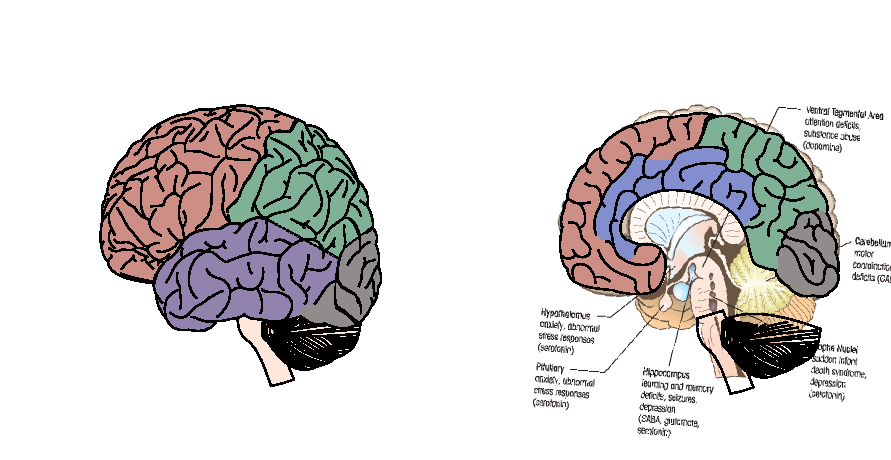
\includegraphics[width=0.8\linewidth]{./img_diagramas/cerebro_zonas.pdf} 
\caption{Referentes fisiológicos usadas para definir a los lóbulos cerebrales. 
Este gráfico será redibujado.
}
\label{lobulos}
\end{figure}

%%%%%%%%%%%%%%%%%%%%%%%%%%%%%%%%%%%%%%%%%%%%%%%%%%%%%%%%%%%%%%%%%%%%%%%%%%%%%%%%%%%%%%%%%%%%%%%%%%%
%%%%%%%%%%%%%%%%%%%%%%%%%%%%%%%%%%%%%%%%%%%%%%%%%%%%%%%%%%%%%%%%%%%%%%%%%%%%%%%%%%%%%%%%%%%%%%%%%%%

\subsection{Electrofisiología}

Usualmente el EEG muestra una actividad oscilatoria continua y cambiante, cuya 
frecuencia var\'ia entre 0.5 y 100 Hz \cite{Clark98}.
Su composici\'on est\'a fuertemente relacionada con el grado de actividad 
cerebral; por ejemplo, hay diferencias claras durante vigilia y sue\~no.
En general la frecuencia del EEG incrementa cuando hay un altos grados de actividad cerebral, lo 
cual se debe a que las ondas se vuelven m\'as as\'incronas, y entonces la magnitud del  potencial 
integrado de superficie decrece (a pesar de la alta actividad cortical).
Aunque la mayor parte del tiempo el EEG es irregular y no muestra patrones claros, es com\'un que 
muestre ondas cerebrales relativamente organizadas llamadas \textbf{ondas cerebrales} que, 
para su estudio, han sido clasificadas en 
cuatro grandes grupos: alfa, beta, gamma, delta.
Estos grupos son ilustrados en la figura \ref{ritmos}.

Debido a que las neuronas en la corteza cerebral tienen orientaciones muy diversas con respecto a 
la superficie y a que disparan de manera asíncrona, el aporte neto de estos campos al potencial 
registrado es casi negligible bajo en condiciones normales, motivo por el cual estas señales son
amplificadas analógicamente antes de ser registradas.
%
Cabe mencionar que ocurre una excepción importante a esta regla cuando se presenta un estímulo
externo, lo cual provoca una respuesta simultánea; estas respuestas suelen tener una amplitud 
relativamente alta y son referidas como \textbf{potenciales evocados}.

\begin{figure}
\centering
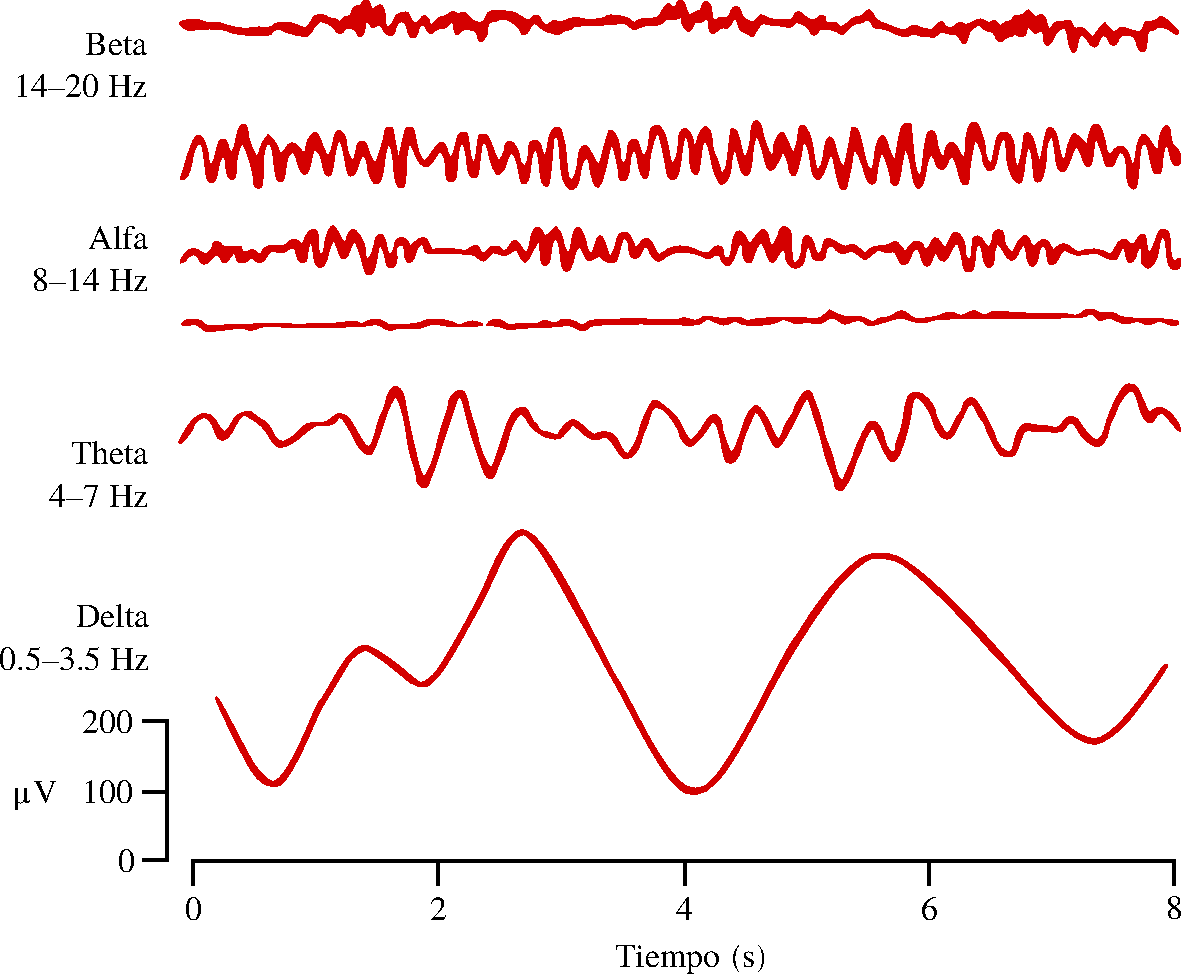
\includegraphics[width=0.55\linewidth]{./img_diagramas/ritmos_hechos.pdf} 
\caption{Ejemplos de ondas cerebrales encontradas en el EEG. Reconstruido de \textit{EEG Signal 
Processing}, por S. Sanei y J. A. Chambers \cite{Sanei07} }
\label{ritmos}
\end{figure}

\begin{description}
\item[Ondas alfa.] Frecuencias entre 8 y 13 Hz. Ocurren en sujetos despiertos en un estado de 
quietud del pensamiento. 
Aparecen m\'as frecuentemente en la regi\'on occipital, pero tambi\'en 
pueden ser registradas en las regiones frontal y parietal. 
%Su voltaje aproximado est\'a entre 20 y 
%200 mV. Cuando el sujeto duerme, las ondas alfa desaparecen completamente. 

\item[Ondas beta.] Frecuencias de 14 a 30 Hz. Normalmente se registran en las regiones parietal y 
frontal. 
%A veces se les divide en dos tipos: beta I y beta II. Las ondas beta I (14--20 Hz) son 
%afectadas por la actividad mental de manera similar a las ondas alfa.
%Las ondas beta II (20--30 Hz), en cambio, aparecen durante una activaci\'on intensa del sistema 
%nervioso central y durante tensi\'on.

\item[Ondas theta.] Frecuencias entre 4 y 7 Hz. Ocurren principalmente en las regiones parietal y 
temporal 
%en ni\~nos, pero pueden aparecer en algunos adultos durante estr\'es emocional, sobre todo 
%durante periodos de decepci\'on y frustraci\'on.

\item[Ondas delta.] Incluye todas las ondas del EEG con frecuencias menores a 3.5 Hz. Ocurren 
generalmente en el sue\~no profundo en infantes, y despu\'es de enfermedades org\'anicas serias del 
cerebro.
\end{description}

Cabe mencionar que el espectro de frecuencias del potencial de campo producido por m\'usculos 
faciales medianamente contra\'idos incluye componentes de frecuencia que bien cuadran en el rango 
usual del EEG (0.5--100 Hz); cuando estas se\~nales 'contaminan' el registro de EEG, son referidas
como \textbf{artefactos}. La variedad de artefactos conocidos es muy basta, al grado de
considerarse a la detecci\'on de \'estos como un paso previo inevitable.

%Para poder comparar los registros obtenidos con múltiples sujetos, conviene claramente usar un
%arreglo estandarizado; 
Respecto al registro \textit{per se}, se define un \textbf{montaje} como
el conjunto de sitios donde se colocan los electrodos y la manera en
que están conecctados entre sí.
%En algunos montajes se conectan los electrodos en serie por pares (bipolar), y el registro 
%representa la diferencia en potencial entre ambos sitios; 
En el montaje usado, uno \textit{referencial}, los electrodos se conectan en paralelo con un 
sitio cuya actividad eléctrica es constante y negligible (los lóbulos de las orejas,
electrodos A1, A2); para el resto de los electrodos se usaron los sitios descritos por el
\textit{International Federation 10--20 system} (\textbf{Sistema 10--20}), propuesto por la 
\textit{International Federation of EEG Societies} \cite{Jasper58,AASM07},
y que se muestran el la figura \ref{img1020}.
El sistema 10--20 usa como referentes principales al \textbf{inion}, protuberancia la región posterior 
del cráneo, el \textbf{nasión}, la unión del hueso frontal y los huesos nasales, y el 
\textbf{punto preauricular}, ubicado arriba del cartílago llamado tragus, que protege el canal 
auditivo \cite{Butkov07}; los sitios se ubican según una cuadrícula construida respecto a las
distancias relativas entre los puntos de referencia.
%Brevemente, el proceso de construcción para los sitios 
%En la figura \ref{img1020} puede verse una representación esquemática
%de la definición de estos sitios, mientras que 
En la figura \ref{corresponde_1020} se muestra de
forma igualmente esquemática las regiones de la corteza cerebral que se corresponden a tales 
sitios --y que a su vez les dan nombre.

\begin{figure}
\centering
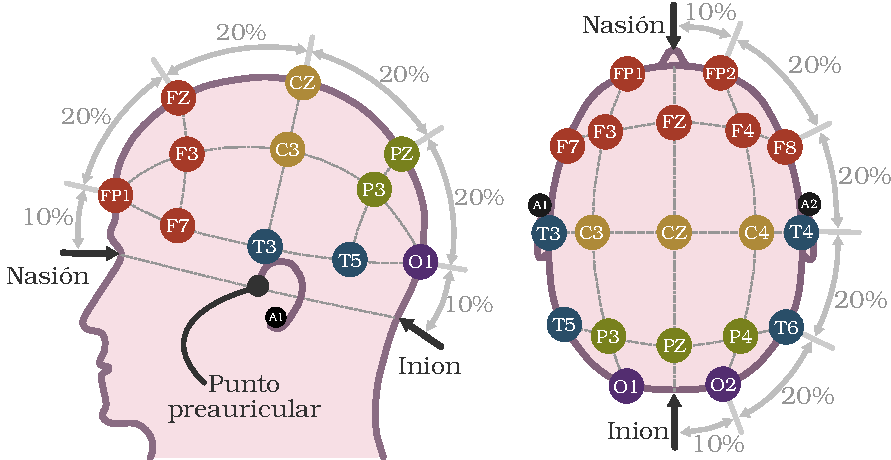
\includegraphics[width=\linewidth]{./img_diagramas/cabeza_proporcionada_color.pdf} 
\caption{Colocación de electrodos según el sistema 10--20.
}
\label{img1020}
\end{figure}

\begin{figure}
\centering
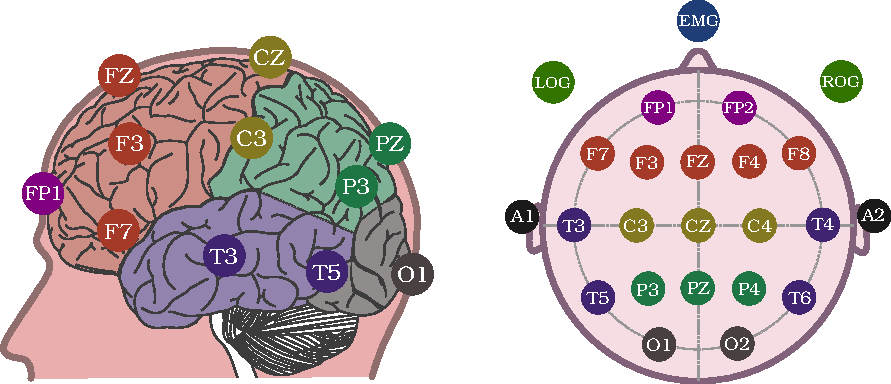
\includegraphics[width=\linewidth]{./img_diagramas/cerebro_1020_v2.pdf} 
\caption{Correspondencia entre el montaje del Sistema 10-20 y las regiones en la corteza cerebral 
que representan
}
\label{corresponde_1020}
\end{figure}

%%%%%%%%%%%%%%%%%%%%%%%%%%%%%%%%%%%%%%%%%%%%%%%%%%%%%%%%%%%%%%%%%%%%%%%%%%%%%%%%%%%%%%%%%%%%%%%%%%%
%%%%%%%%%%%%%%%%%%%%%%%%%%%%%%%%%%%%%%%%%%%%%%%%%%%%%%%%%%%%%%%%%%%%%%%%%%%%%%%%%%%%%%%%%%%%%%%%%%%

\subsection{Polisomnografía}

Se entiende al \textbf{sueño} como un proceso vital cíclico complejo y activo, compuesto por 
varias fases y que posee una estructura interna característica, con diversas interrelaciones en los 
sistemas hormonales y nerviosos \cite{FernandezConde07}.
Para el ser humano se puede caracterizar por las siguientes propiedades \cite{CarrilloMora}:
\begin{enumerate}
\item Disminución de conciencia y reactividad a estímulos externos
\item Fácilmente reversible, lo cual lo diferencia de otros estados patológicos como el estupor y 
el coma
\item Inmovilidad y relajación muscular
\item Periodicidad típica circadiana (diaria)
\item Los individuos adquieren una postura estereotipada
\item La privación induce alteraciones conductuales y 
fisiológicas, además de que genera una \textit{deuda} acumulativa
\end{enumerate}

El sueño normal se divide en dos etapas principales: MOR (fase R) y NMOR (fase N), que se 
diferencian por sus rasgos electroencefalográficos y una serie de características fisiológicas, y 
de los cuales obtienen sus nombres.
Cabe mencionar que la nomenclatura acerca de las fases del sue\~no ha sido recientemente modificada 
por la American Association of Sleep Medicine (AASM) en 2007 \cite{AASM07}, de modo que en este 
trabajo se  usar\'an ambas nomenclaturas siempre que sea posible, por fines de compatibilidad.

Durante el sue\~no MOR (fase R), ocurre que las ondas lentas y amplitud alta son reemplazadas por 
ondas r\'apidas de bajo voltaje, irregulares, y que recuerdan la actividad en el EEG durante el 
estado de alerta.
La presencia de estos patrones irregulares no interrumpen el sue\~no, sino que incrementan el 
umbral para los est\'imulos externos; este comportamiento es referido como 'sue\~no parad\'ojico'.
Durante esta etapa de sue\~no, el sujeto exhibe movimientos oculares r\'apidos (MOR), raz\'on por 
la cual recibe su nombre caracter\'istico.
Durante el sue\~no MOR se producen la mayor\'ia de las enso\~naciones (referidos coloquialmente 
como sue\~nos), y la mayor\'ia de los pacientes que despiertan durante esta fase suelen recordar 
v\'ividamente el contenido de sus enso\~naciones \cite{Chokroverty09}.
F\'isicamente el tono de todos los m\'usculos disminuye (con excepci\'on de los m\'usculos 
respiratorios y los esf\'interes vesical y anal), as\'i mismo la frecuencia cardiaca y respiratoria 
se vuelve irregular.

El sue\~no fuera de la etapa MOR es referido como no-MOR (NMOR, fase N), y es dividido en etapas 
seg\'un la 'profundidad' del sue\~no, entendida en t\'erminos de la actividad cerebral registrada.
En el sue\~no profundo se observan ondas delta muy irregulares, y junto con ellas ocurren trenes 
cortos de ondas, parecidas a las alfa, y que son referidas como \textit{husos de sue\~no}. 
El ritmo alfa y los husos de sue\~no est\'an sincronizados en el sue\~no y la somnolencia, en 
contraste con la actividad irregular, desincronizada y de bajo voltaje registrada en estado de 
alerta.
A grosso modo, la clasificaci\'on de etapas del sue\~no seg\'un la AASM se basa en las siguientes
caracter\'isticas \cite{Hori01}:

\begin{description}
\item[Vigilia (W)] Presencia de ritmo alfa contin\'uo con m\'axima amplitud sobre regiones de la 
corteza parieto-occipital. Tono muscular relativamente alto y ausencia de movimientos oculares.

\item[Fase 1 (N1)] Corresponde con la somnolencia o el inicio del sue\~no ligero, en ella es muy 
f\'acil despertarse. 
Presencia intermitente de ondas alfa en menos del 50\% de la \'epoca, actividad de frecuencias 
mezcladas y bajo voltaje, adem\'as de movimientos oculares lentos y algunas ondas agudas. 
La actividad muscular disminuye paulatinamente, pueden observarse sacudidas musculares s\'ubitas 
que a veces coinciden con una sensaci\'on de ca\'ida. 

\item[Fase 2 (N2)] Se caracteriza por patrones espec\'ificos de actividad cerebral conocidos como 
husos de sue\~no y complejos K. 
Puede aparecer hasta un 20\% de ondas lentas (ritmo delta). Ausencia de actividad ocular y tono 
muscular bajo.
La temperatura, la frecuencia card\'iaca y respiratoria disminuyen paulatinamente. 

\item[Fases 3 (N3)] Predominan ondas de frecuencias muy bajas ($<2$ Hz) con amplitudes superiores a 
75 $\mu$V en m\'as del 20\% y menos del 50\% de la \'epoca. Pueden tambi\'en aparecer complejos K y 
husos de sue\~no de forma espor\'adica. Ausencia de actividad ocular y tono muscular bajo.

\item[Fase 4 (N4)] La fase m\'as profunda del sue\~no NMOR y referido como 'sue\~no de ondas 
lentas', pues hay presencia de \'estas ondas en m\'as del 50\% de la \'epoca. Las dem\'as 
caracter\'isticas son similares a las de la fase 3.

\item[Fase MOR (R)] Presencia de actividad EEG de baja amplitud y frecuencias entremezcladas 
(theta-alfa-beta) similar a la observada en el estado de vigilia activa con ojos abiertos.
\end{description}

Un adulto joven pasa aproximadamente entre 70--100 minutos en el sue\~no NMOR para despu\'es entrar 
al sue\~no MOR, el cual puede durar entre 5--30 min; este ciclo se repite cada hora y media.
En los ancianos se va fragmentando el sue\~no nocturno con frecuentes episodios de despertar, se 
reduce mucho el porcentaje de sue\~no en fase 4, pero se mantiene constante el porcentaje de 
sue\~no MOR. Adicionalmente, muchos adultos mayores dormitan durante el d\'ia varias siestas cortas 
\cite{CarrilloMora}.

La edad es un factor decisivo para la cantidad de horas de sueño. El recién nacido duerme entre 14 y 18 horas, el lactante entre 12 y 14 horas, el niño en etapa escolar entre 11 y 12 horas y en la edad adulta, la mayoría duerme entre 7 y 8 horas por noche. En otras palabras, es fisiológico que el número de horas dormidas vaya disminuyendo progresivamente a lo largo de la vida, pudiendo existir una diferencia de hasta 16 horas como promedio entre la niñez y la edad adulta. En los ancianos, el número de horas de diferencia entre las horas de sueño propias v/s las horas de sueño de la niñez, es aún mayor

\cite{Contreras13}

\begin{figure}
\centering
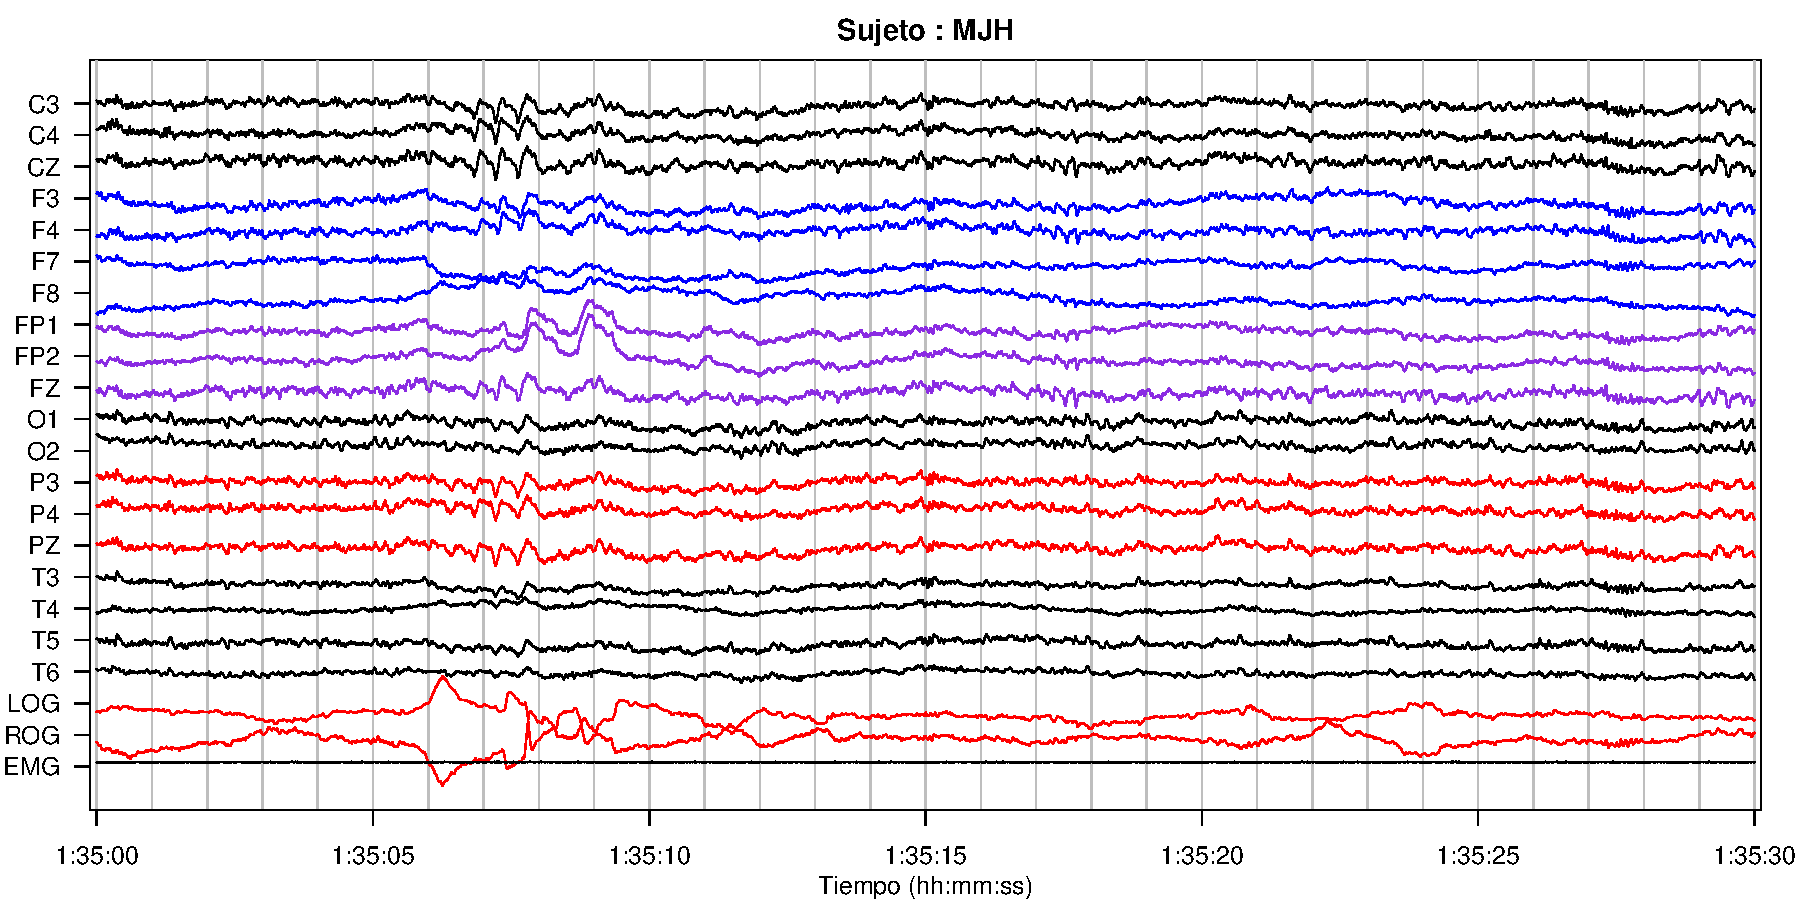
\includegraphics[width=\linewidth]
{./img_ejemplos/MJH_190_PDG_lucirse_PSG.pdf}
\caption{Registro de PSG en el sujeto MJH durante sue\~no MOR. 
%N\'otese que el canal EMG permanece 
%silente (indicativo de aton\'ia muscular) mientras que los canales ROG y LOG exhiben actividad de 
%gran amplitud y sincronizaci\'on (movimientos oculares r\'apidos), caracter\'isticas indicativas de
%la etapa de sue\~no.
}
\label{ejemplos_mor}
\end{figure}

%textwidth: \printinunitsof{cm}\prntlen{\textwidth}
%
%linewidth: \printinunitsof{cm}\prntlen{\linewidth}

%%%%%%%%%%%%%%%%%%%%%%%%%%%%%%%%%%%%%%%%%%%%%%%%%%%%%%%%%%%%%%%%%%%%%%%%%%%%%%%%%%%%%%%%%%%%%%%%%%%
%%%%%%%%%%%%%%%%%%%%%%%%%%%%%%%%%%%%%%%%%%%%%%%%%%%%%%%%%%%%%%%%%%%%%%%%%%%%%%%%%%%%%%%%%%%%%%%%%%%
%%%%%%%%%%%%%%%%%%%%%%%%%%%%%%%%%%%%%%%%%%%%%%%%%%%%%%%%%%%%%%%%%%%%%%%%%%%%%%%%%%%%%%%%%%%%%%%%%%%
%%%%%%%%%%%%%%%%%%%%%%%%%%%%%%%%%%%%%%%%%%%%%%%%%%%%%%%%%%%%%%%%%%%%%%%%%%%%%%%%%%%%%%%%%%%%%%%%%%%
